\documentclass[]{article}
\usepackage{lmodern}
\usepackage{amssymb,amsmath}
\usepackage{ifxetex,ifluatex}
\usepackage{fixltx2e} % provides \textsubscript
\ifnum 0\ifxetex 1\fi\ifluatex 1\fi=0 % if pdftex
  \usepackage[T1]{fontenc}
  \usepackage[utf8]{inputenc}
\else % if luatex or xelatex
  \ifxetex
    \usepackage{mathspec}
  \else
    \usepackage{fontspec}
  \fi
  \defaultfontfeatures{Ligatures=TeX,Scale=MatchLowercase}
\fi
% use upquote if available, for straight quotes in verbatim environments
\IfFileExists{upquote.sty}{\usepackage{upquote}}{}
% use microtype if available
\IfFileExists{microtype.sty}{%
\usepackage{microtype}
\UseMicrotypeSet[protrusion]{basicmath} % disable protrusion for tt fonts
}{}
\usepackage[margin=1in]{geometry}
\usepackage{hyperref}
\hypersetup{unicode=true,
            pdfauthor={Geovan},
            pdfborder={0 0 0},
            breaklinks=true}
\urlstyle{same}  % don't use monospace font for urls
\usepackage{color}
\usepackage{fancyvrb}
\newcommand{\VerbBar}{|}
\newcommand{\VERB}{\Verb[commandchars=\\\{\}]}
\DefineVerbatimEnvironment{Highlighting}{Verbatim}{commandchars=\\\{\}}
% Add ',fontsize=\small' for more characters per line
\newenvironment{Shaded}{}{}
\newcommand{\AlertTok}[1]{\textcolor[rgb]{1.00,0.00,0.00}{\textbf{#1}}}
\newcommand{\AnnotationTok}[1]{\textcolor[rgb]{0.38,0.63,0.69}{\textbf{\textit{#1}}}}
\newcommand{\AttributeTok}[1]{\textcolor[rgb]{0.49,0.56,0.16}{#1}}
\newcommand{\BaseNTok}[1]{\textcolor[rgb]{0.25,0.63,0.44}{#1}}
\newcommand{\BuiltInTok}[1]{#1}
\newcommand{\CharTok}[1]{\textcolor[rgb]{0.25,0.44,0.63}{#1}}
\newcommand{\CommentTok}[1]{\textcolor[rgb]{0.38,0.63,0.69}{\textit{#1}}}
\newcommand{\CommentVarTok}[1]{\textcolor[rgb]{0.38,0.63,0.69}{\textbf{\textit{#1}}}}
\newcommand{\ConstantTok}[1]{\textcolor[rgb]{0.53,0.00,0.00}{#1}}
\newcommand{\ControlFlowTok}[1]{\textcolor[rgb]{0.00,0.44,0.13}{\textbf{#1}}}
\newcommand{\DataTypeTok}[1]{\textcolor[rgb]{0.56,0.13,0.00}{#1}}
\newcommand{\DecValTok}[1]{\textcolor[rgb]{0.25,0.63,0.44}{#1}}
\newcommand{\DocumentationTok}[1]{\textcolor[rgb]{0.73,0.13,0.13}{\textit{#1}}}
\newcommand{\ErrorTok}[1]{\textcolor[rgb]{1.00,0.00,0.00}{\textbf{#1}}}
\newcommand{\ExtensionTok}[1]{#1}
\newcommand{\FloatTok}[1]{\textcolor[rgb]{0.25,0.63,0.44}{#1}}
\newcommand{\FunctionTok}[1]{\textcolor[rgb]{0.02,0.16,0.49}{#1}}
\newcommand{\ImportTok}[1]{#1}
\newcommand{\InformationTok}[1]{\textcolor[rgb]{0.38,0.63,0.69}{\textbf{\textit{#1}}}}
\newcommand{\KeywordTok}[1]{\textcolor[rgb]{0.00,0.44,0.13}{\textbf{#1}}}
\newcommand{\NormalTok}[1]{#1}
\newcommand{\OperatorTok}[1]{\textcolor[rgb]{0.40,0.40,0.40}{#1}}
\newcommand{\OtherTok}[1]{\textcolor[rgb]{0.00,0.44,0.13}{#1}}
\newcommand{\PreprocessorTok}[1]{\textcolor[rgb]{0.74,0.48,0.00}{#1}}
\newcommand{\RegionMarkerTok}[1]{#1}
\newcommand{\SpecialCharTok}[1]{\textcolor[rgb]{0.25,0.44,0.63}{#1}}
\newcommand{\SpecialStringTok}[1]{\textcolor[rgb]{0.73,0.40,0.53}{#1}}
\newcommand{\StringTok}[1]{\textcolor[rgb]{0.25,0.44,0.63}{#1}}
\newcommand{\VariableTok}[1]{\textcolor[rgb]{0.10,0.09,0.49}{#1}}
\newcommand{\VerbatimStringTok}[1]{\textcolor[rgb]{0.25,0.44,0.63}{#1}}
\newcommand{\WarningTok}[1]{\textcolor[rgb]{0.38,0.63,0.69}{\textbf{\textit{#1}}}}
\usepackage{longtable,booktabs}
\usepackage{graphicx,grffile}
\makeatletter
\def\maxwidth{\ifdim\Gin@nat@width>\linewidth\linewidth\else\Gin@nat@width\fi}
\def\maxheight{\ifdim\Gin@nat@height>\textheight\textheight\else\Gin@nat@height\fi}
\makeatother
% Scale images if necessary, so that they will not overflow the page
% margins by default, and it is still possible to overwrite the defaults
% using explicit options in \includegraphics[width, height, ...]{}
\setkeys{Gin}{width=\maxwidth,height=\maxheight,keepaspectratio}
\IfFileExists{parskip.sty}{%
\usepackage{parskip}
}{% else
\setlength{\parindent}{0pt}
\setlength{\parskip}{6pt plus 2pt minus 1pt}
}
\setlength{\emergencystretch}{3em}  % prevent overfull lines
\providecommand{\tightlist}{%
  \setlength{\itemsep}{0pt}\setlength{\parskip}{0pt}}
\setcounter{secnumdepth}{0}
% Redefines (sub)paragraphs to behave more like sections
\ifx\paragraph\undefined\else
\let\oldparagraph\paragraph
\renewcommand{\paragraph}[1]{\oldparagraph{#1}\mbox{}}
\fi
\ifx\subparagraph\undefined\else
\let\oldsubparagraph\subparagraph
\renewcommand{\subparagraph}[1]{\oldsubparagraph{#1}\mbox{}}
\fi

%%% Use protect on footnotes to avoid problems with footnotes in titles
\let\rmarkdownfootnote\footnote%
\def\footnote{\protect\rmarkdownfootnote}

%%% Change title format to be more compact
\usepackage{titling}

% Create subtitle command for use in maketitle
\providecommand{\subtitle}[1]{
  \posttitle{
    \begin{center}\large#1\end{center}
    }
}

\setlength{\droptitle}{-2em}

  \title{}
    \pretitle{\vspace{\droptitle}}
  \posttitle{}
    \author{Geovan}
    \preauthor{\centering\large\emph}
  \postauthor{\par}
      \predate{\centering\large\emph}
  \postdate{\par}
    \date{18/06/2020}


\begin{document}

So, I am an enthusiastic of R programming since about one year ago, when
I started to use it for statistical purposes. Since then, I've been
trying to spread the benefits of using R for hypothesis testing and data
visualization.

Not rarely, we have to test our variables for normality, specially to
make a decision about what inferential test to use (parametric or
nonparametric). Attempting to help other R beginners who are aiming to
check the normality of their data, I decided to make available a simple
function I had built due to a lab demand. This function is a way to
easily know which variables from a given dataset have a normal (or not
normal) distribution. In this post I will show you how it works and how
to use it.

\begin{itemize}
\tightlist
\item
  \textbf{Loading the function}
\end{itemize}

The function is called \texttt{whos\_norm} and can be found on my
\href{https://github.com/geovanjr/stats}{Github}. Alternatively, you can
load the function to your environment, simply running:

\begin{Shaded}
\begin{Highlighting}[]
\KeywordTok{source}\NormalTok{(}\StringTok{'https://github.com/geovanjr/stats/raw/master/whos_norm.R'}\NormalTok{)}
\end{Highlighting}
\end{Shaded}

Function loaded, we can start to play.

At first, you can notice that \texttt{whos\_norm} has just only one
argument, \texttt{data}, what make its use quite easy. Literally, you
just have to put your dataset and run.

To illustrate, I'll use the \texttt{iris} dataset. But before we use the
function itself, let's take a look on the \texttt{iris} data.

\begin{Shaded}
\begin{Highlighting}[]
\KeywordTok{library}\NormalTok{(tidyverse)}

\KeywordTok{glimpse}\NormalTok{(iris)}
\end{Highlighting}
\end{Shaded}

\begin{verbatim}
## Observations: 150
## Variables: 5
## $ Sepal.Length <dbl> 5.1, 4.9, 4.7, 4.6, 5.0, 5.4, 4.6, 5.0, 4.4, 4.9,...
## $ Sepal.Width  <dbl> 3.5, 3.0, 3.2, 3.1, 3.6, 3.9, 3.4, 3.4, 2.9, 3.1,...
## $ Petal.Length <dbl> 1.4, 1.4, 1.3, 1.5, 1.4, 1.7, 1.4, 1.5, 1.4, 1.5,...
## $ Petal.Width  <dbl> 0.2, 0.2, 0.2, 0.2, 0.2, 0.4, 0.3, 0.2, 0.2, 0.1,...
## $ Species      <fct> setosa, setosa, setosa, setosa, setosa, setosa, s...
\end{verbatim}

We can see that \texttt{iris} data has 150 observations regarding 4
numeric variables (\texttt{Sepal.Length}, \texttt{Sepal.Width},
\texttt{Petal.Length} and \texttt{Petal.Width}) and one factor
(\texttt{Species}), which levels stand for the iris species.

\begin{itemize}
\tightlist
\item
  \textbf{Using \texttt{whos\_norm}}
\end{itemize}

Now, using the function, we can look for the normality of \texttt{iris}'
variables:

\begin{Shaded}
\begin{Highlighting}[]
\KeywordTok{whos_norm}\NormalTok{(iris)}
\end{Highlighting}
\end{Shaded}

\begin{verbatim}
## $all
##       variable     W      p signif
## 1 Sepal.Length 0.976 0.0102      *
## 2  Sepal.Width 0.985 0.1012 normal
## 3 Petal.Length 0.876 0.0000      *
## 4  Petal.Width 0.902 0.0000      *
## 
## $normal
##      variable     W      p signif
## 1 Sepal.Width 0.985 0.1012 normal
## 
## $not_normal
##       variable     W      p signif
## 1 Sepal.Length 0.976 0.0102      *
## 2 Petal.Length 0.876 0.0000      *
## 3  Petal.Width 0.902 0.0000      *
\end{verbatim}

The output of \texttt{whos\_norm} comprise a list of three elements:
\texttt{all}, \texttt{normal} and \texttt{not\_normal}. As the names
suggest, the first one shows all the variables assessed, the second one
shows only normal while the third shows only non-normal variables. Both
shows the variables name and the related statistic. At this point, I
have to say that the assessment of normality is based on the
Shapiro-Wilk test (\texttt{shapiro.test}), so the \texttt{W} and the
\texttt{p}-value is referent to this test. In a near future I should add
an argument to choose an evaluation based on Shapiro-Wilk or
Kolmogorov-Smirnov test.

Interpreting the output, we can easily see that only
\texttt{Sepal.Width} has a normal distribution, while
\texttt{Sepal.Length}, \texttt{Petal.Length} and \texttt{Petal.Width}
both do not. We can check this looking for its density and Q-Q plot:

\begin{center}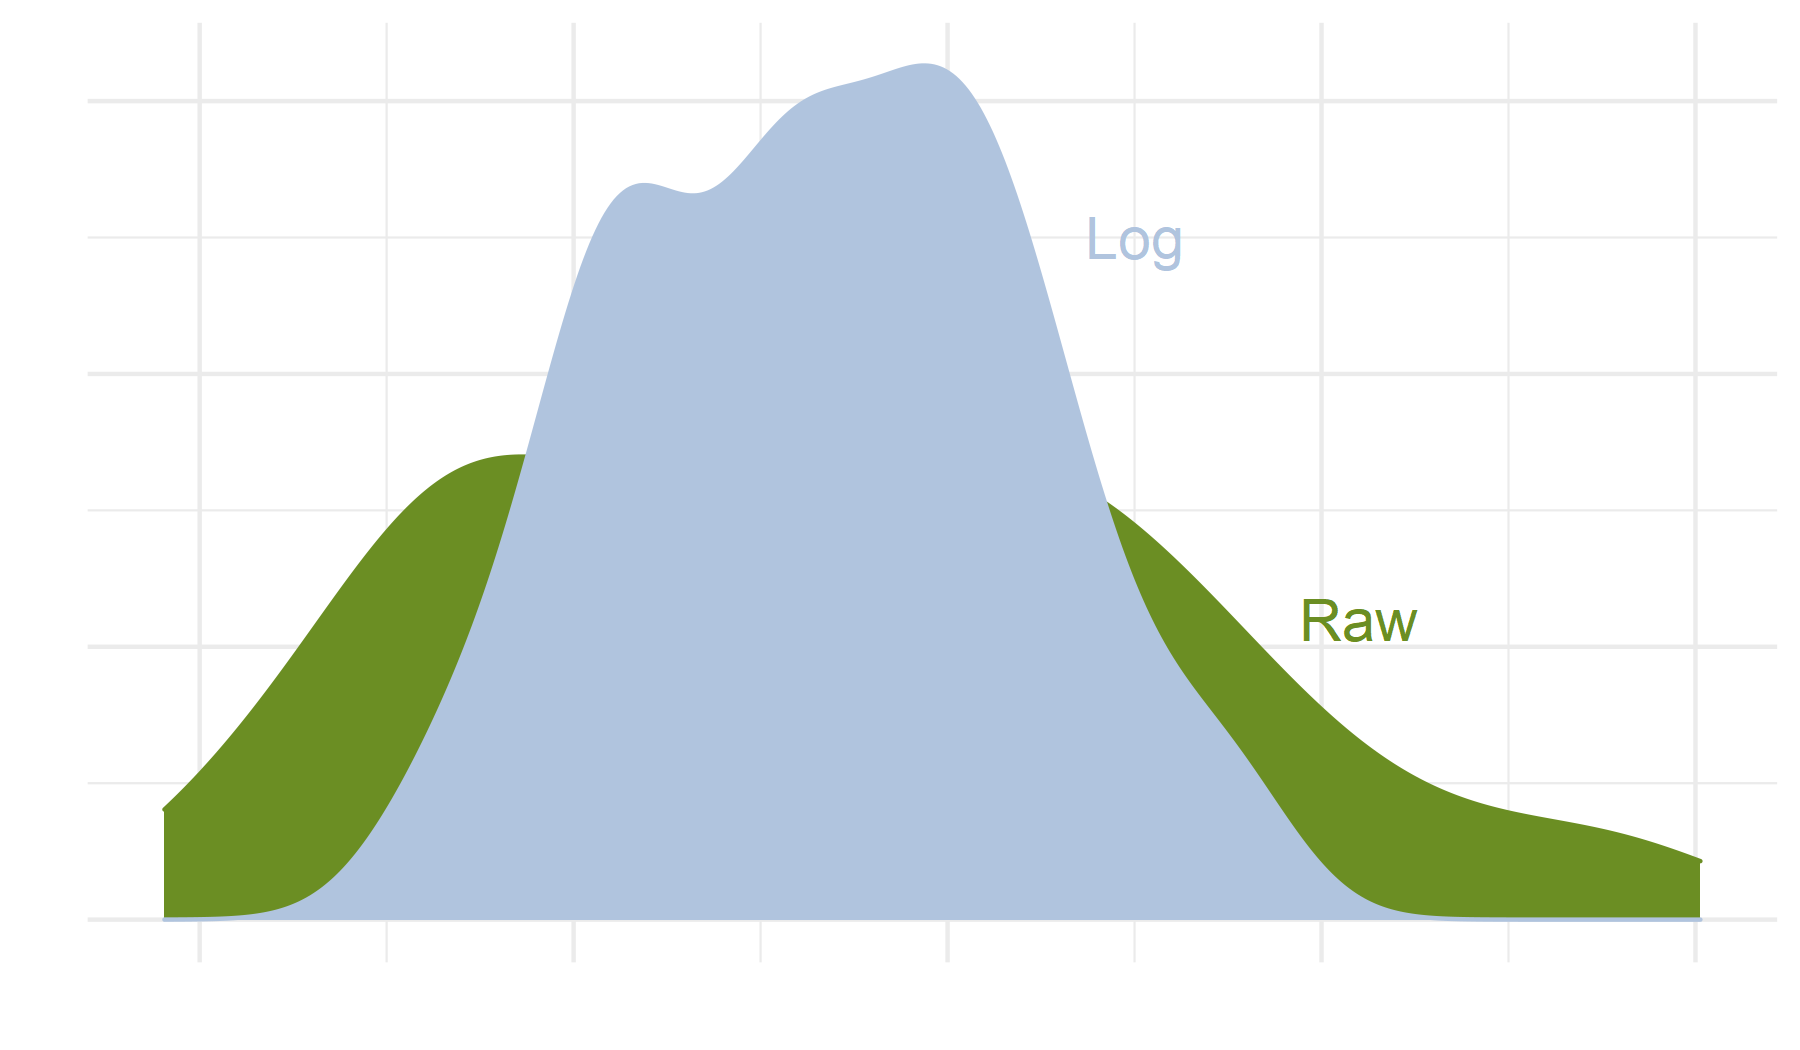
\includegraphics{A-funtion-for-easy-assessment-of-variable-normality_files/figure-latex/unnamed-chunk-5-1} \end{center}

\begin{itemize}
\tightlist
\item
  \textbf{Dealing with factor variables}
\end{itemize}

You may have noticed that \texttt{Species} is not outputed, as expected,
since it is a factor. It is because \texttt{whos\_norm} identify which
variables are factors and exclude it from \texttt{shapiro.test}, so you
don't have to worry about subsetting your data to numerical variables.

\begin{itemize}
\tightlist
\item
  \textbf{Assessing output elements}
\end{itemize}

Maybe you are a person who like quiet outputs. In this case, you can
save \texttt{whos\_norm} output into an object and assess only the
element you want:

\begin{Shaded}
\begin{Highlighting}[]
\NormalTok{normality_assess <-}\StringTok{ }\KeywordTok{whos_norm}\NormalTok{(iris)}

\NormalTok{normality_assess}\OperatorTok{$}\NormalTok{not_normal }\CommentTok{# seeing just non-normal variables}
\end{Highlighting}
\end{Shaded}

\begin{longtable}[]{@{}lrrl@{}}
\toprule
variable & W & p & signif\tabularnewline
\midrule
\endhead
Sepal.Length & 0.976 & 0.0102 & *\tabularnewline
Petal.Length & 0.876 & 0.0000 & *\tabularnewline
Petal.Width & 0.902 & 0.0000 & *\tabularnewline
\bottomrule
\end{longtable}

Still, if you do not like your environment full of objects, you can call
the output element whithout the need of saving it:

\begin{Shaded}
\begin{Highlighting}[]
\KeywordTok{whos_norm}\NormalTok{(iris)}\OperatorTok{$}\NormalTok{normal}
\end{Highlighting}
\end{Shaded}

\begin{longtable}[]{@{}lrrl@{}}
\toprule
variable & W & p & signif\tabularnewline
\midrule
\endhead
Sepal.Width & 0.985 & 0.1012 & normal\tabularnewline
\bottomrule
\end{longtable}

\begin{itemize}
\tightlist
\item
  \textbf{Data structure compatibilities}
\end{itemize}

Regarding data structure, \texttt{whos\_norm} works with \texttt{tibble}
and \texttt{data.frame}, but not with \texttt{matrix}.

\begin{itemize}
\tightlist
\item
  \textbf{Requirements}
\end{itemize}

To finish my brief post, I must say something about the requirements of
\texttt{whos\_norm}. Actually, only \texttt{dplyr} package is required,
once \texttt{shapiro.test} function is a built-in. You can load
\texttt{dplyr} or \texttt{tidyverse} before running the
\texttt{whos\_norm} or, if you already have one of these packages
installed, the function will call for them when running.

That's all, folks.


\end{document}
